\begin{frame}{Adjoint Method}
    \begin{itemize}
        \item Airfoil optimization
        \item Require primal and adjoint simulation
        \item Complexity is independent of the number of parameters (eg control points on the airfoil)
    \end{itemize}

\end{frame}


\begin{frame}{NACA0012 $AoA=\ang{2.5}$, $Re=1000$ - drag minimization}
    \begin{figure}[h]
        \centering
        \begin{subfigure}[h]{0.45\textwidth}
            \centering
            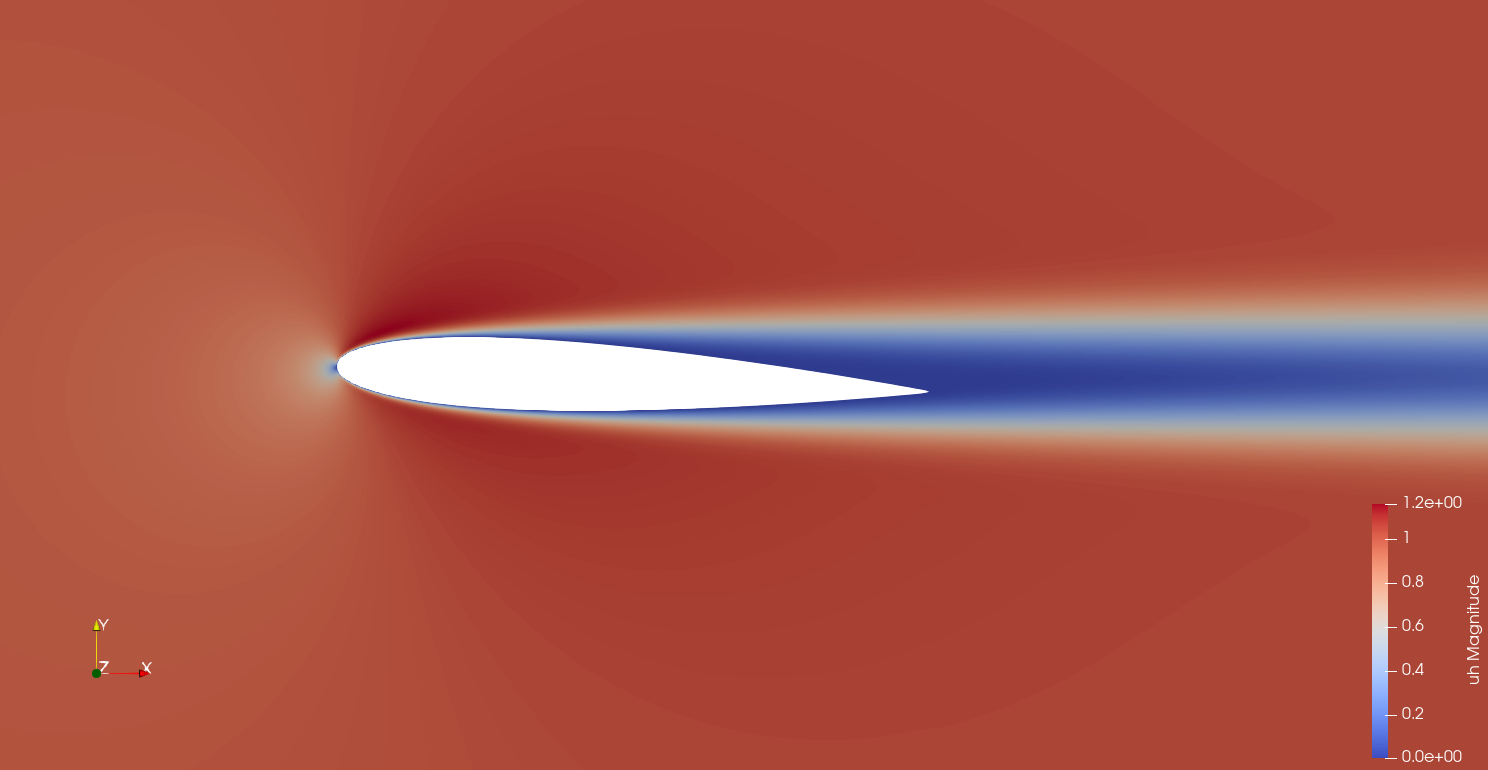
\includegraphics[width=\textwidth]{NACA0012_Uprimal.png}
        \end{subfigure}
        \hfill
        \begin{subfigure}[h]{0.45\textwidth}
            \centering
            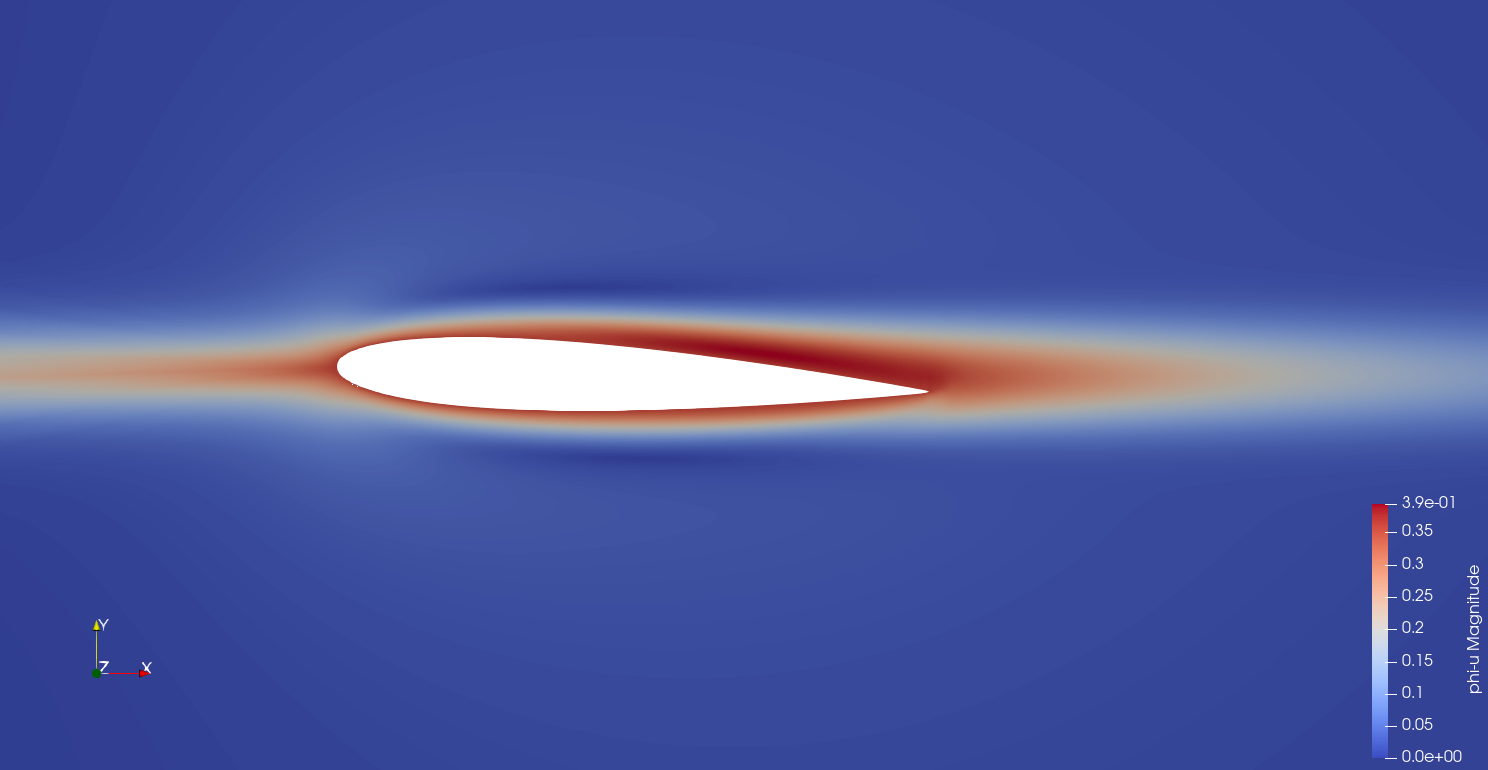
\includegraphics[width=\textwidth]{NACA0012_Uadjoint.png}
        \end{subfigure}
        \caption{Primal and Adjoint Velocity}
    \end{figure}
\end{frame}



\begin{frame}{NACA0012 $AoA=\ang{2.5}$, $Re=1000$ - drag minimization}
    \begin{figure}[h]
        \centering
        \begin{subfigure}[h]{0.45\textwidth}
            \centering
            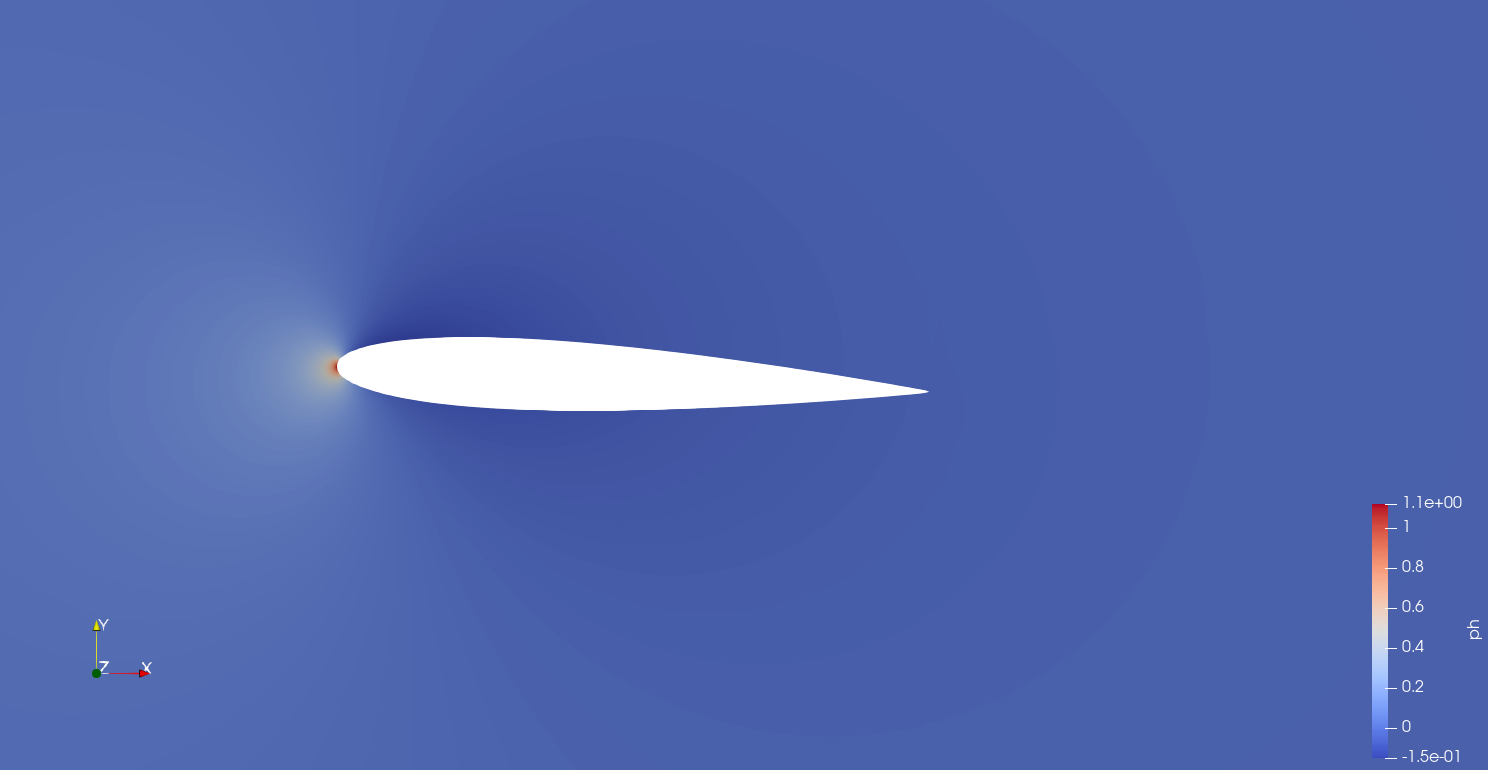
\includegraphics[width=\textwidth]{NACA0012_Pprimal.png}
        \end{subfigure}
        \hfill
        \begin{subfigure}[h]{0.45\textwidth}
            \centering
            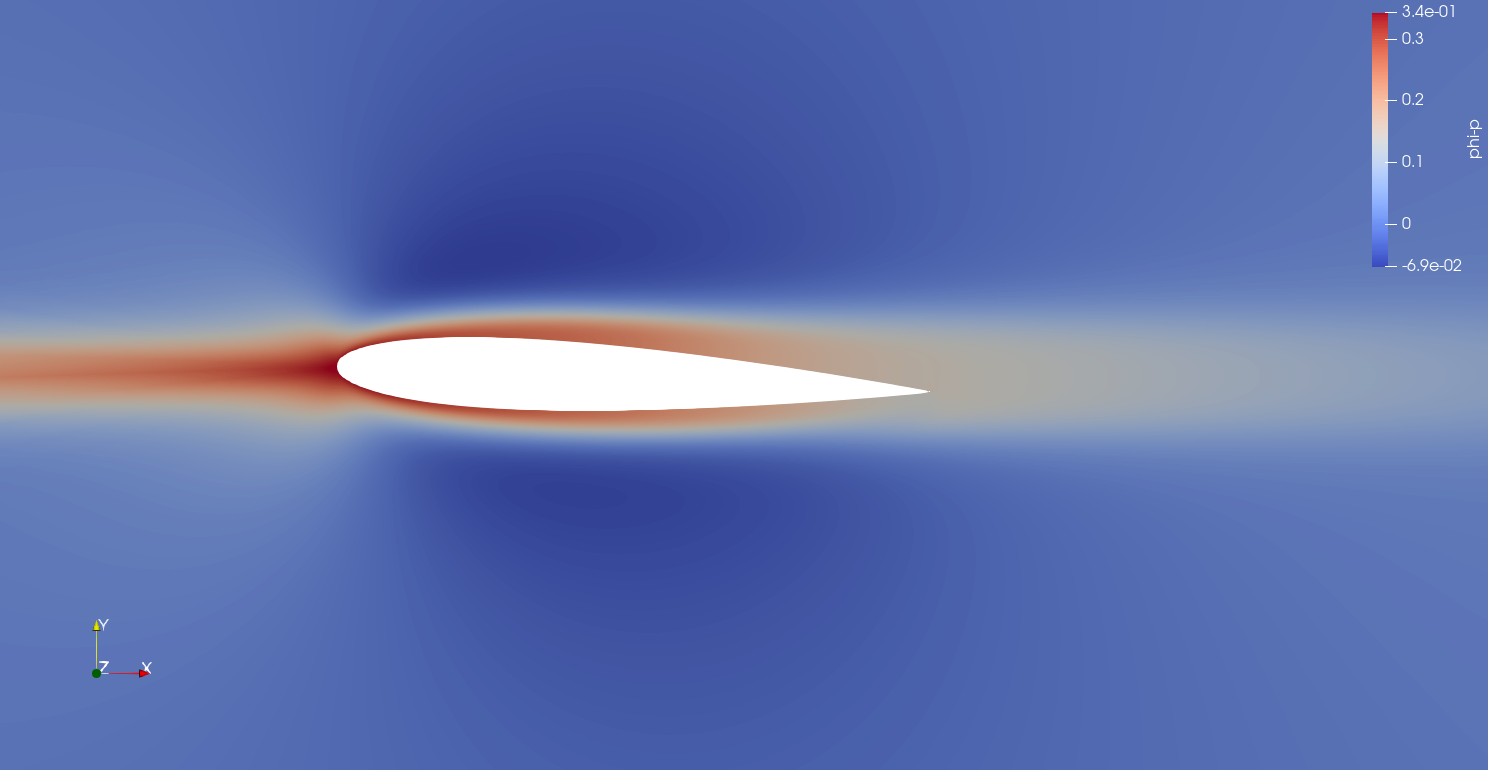
\includegraphics[width=\textwidth]{NACA0012_Padjoint.png}
        \end{subfigure}
        \caption{Primal and Adjoint pressure}
    \end{figure}
\end{frame}


\begin{frame}{NACA0012 $AoA=\ang{0.0}$, $Re=100$ - drag minimization}
    \begin{figure}[h]
        \centering
        \begin{subfigure}[h]{0.45\textwidth}
            \centering
            \includegraphics[width=\textwidth]{MeshDeformation.png}
            \caption{Local Mesh Deformation}
        \end{subfigure}
        \hfill
        \begin{subfigure}[h]{0.45\textwidth}
            \centering
            \includegraphics[width=\textwidth]{Adjoint_FD.pdf}
        \end{subfigure}
        \caption{Finite Difference and Adjoint gradient}
    \end{figure}
\end{frame}